
% Group addresses by affiliation; use superscriptaddress for long
% author lists, or if there are many overlapping affiliations.
% For Phys. Rev. appearance, change preprint to twocolumn.
% Choose pra, prb, prc, prd, pre, prl, prstab, prstper, or rmp for journal
%  Add 'draft' option to mark overfull boxes with black boxes
%  Add 'showpacs' option to make PACS codes appear
%  Add 'showkeys' option to make keywords appear
\documentclass[aps,prl,preprint,groupedaddress]{revtex4-1}
%\documentclass[aps,prl,preprint,superscriptaddress]{revtex4-1}
%\documentclass[aps,prl,reprint,groupedaddress]{revtex4-1}
\usepackage{bm}
\usepackage{amsmath}
\usepackage{graphicx}

% You should use BibTeX and apsrev.bst for references
% Choosing a journal automatically selects the correct APS
% BibTeX style file (bst file), so only uncomment the line
% below if necessary.
%\bibliographystyle{apsrev4-1}

\begin{document}
\graphicspath{{../images/}}

% Use the \preprint command to place your local institutional report
% number in the upper righthand corner of the title page in preprint mode.
% Multiple \preprint commands are allowed.
% Use the 'preprintnumbers' class option to override journal defaults
% to display numbers if necessary
%\preprint{}

%Title of paper
\title{$N_{\text{eff}}$ priors}

% repeat the \author .. \affiliation  etc. as needed
% \email, \thanks, \homepage, \altaffiliation all apply to the current
% author. Explanatory text should go in the []'s, actual e-mail
% address or url should go in the {}'s for \email and \homepage.
% Please use the appropriate macro foreach each type of information

% \affiliation command applies to all authors since the last
% \affiliation command. The \affiliation command should follow the
% other information
% \affiliation can be followed by \email, \homepage, \thanks as well.
\author{}
%\email[]{Your e-mail address}
%\homepage[]{Your web page}
%\thanks{}
%\altaffiliation{}
\affiliation{}

%Collaboration name if desired (requires use of superscriptaddress
%option in \documentclass). \noaffiliation is required (may also be
%used with the \author command).
%\collaboration can be followed by \email, \homepage, \thanks as well.
%\collaboration{}
%\noaffiliation

\date{\today}

\begin{abstract}
Try to understand the effect of priors on different parameters on the $N_{\text{eff}}$ errors with a Fisher matrix approach. Where should you invest time and money if you really care about the value of $N_{\text{eff}}$?

\begin{itemize}
\item We are now using a simplistic lensing noise but I have lensing noise with the usual Hu Okamoto formula. Iterative Seljack not there yet.
\item We are varying $\tau, ~ n_{s}, ~ A_{s}, ~ N_{\rm eff}, ~ H_{0}, w,~\Omega_{\nu}h^{2},~\Omega_{c}h^{2},~\Omega_{b}h^{2}$. The neutrino sector consists of one massive neutrino of $m_{\nu}=0.083$ eV, $\Omega_{\nu}h^{2}=0.0009$
\item Next TODO: Check for bugs and errors code in its early stages. PCA? what prior is more important? Full MCMC should not be extremely hard with cosmosis.
\end{itemize}


\end{abstract}

% insert suggested PACS numbers in braces on next line
\pacs{}
% insert suggested keywords - APS authors don't need to do this
%\keywords{}

%\maketitle must follow title, authors, abstract, \pacs, and \keywords
\maketitle

% body of paper here - Use proper section commands
% References should be done using the \cite, \ref, and \label commands
\section{Introduction}


% Put \label in argument of \section for cross-referencing
%\section{\label{}}
\subsection{}
\subsubsection{}

\section{Theory}

\subsection{Fisher Matrix formalism}
Copied from paper change it for pubblication:

To avoid any possible numerical instability in the marginalising procedure, we calculate the the Fisher matrix marginalised over the standard LCDM parameters following (Albrecht et al. 2009)
\begin{equation}
G = F^{\phi\phi} - F^{\phi\psi}U\Lambda^{-1}U^{T}F^{\phi\psi},
\end{equation}
where we define $\phi = \{N_{eff},...\}$ and $\psi = \{\Omega_{m} ... marginal\}$; therefore, $F^{\phi\phi}$ is the block of the total Fisher matrix containing the parameters we want to constrain, whilst $F^{\psi\psi}$ is the nuisance-parameter Fisher sub-matrix. Here, $\Lambda$ is the diagonal matrix whose elements are the eigenvalues of $F^{\psi\psi}$, whilst U is the orthogonal matrix diagonalising $F^{\psi\psi}$. By using Eq., our marginalising procedure is more stable, since degeneracies in $F^{\phi\phi}$ are properly propagated to G with no instabilities, and we do not even worry about a possibly ill-conditioned $F^{\phi\phi}$ sub-matrix, since we check its stability on the fly by the diagonalisation.


\begin{figure}[htbp]
\begin{center}
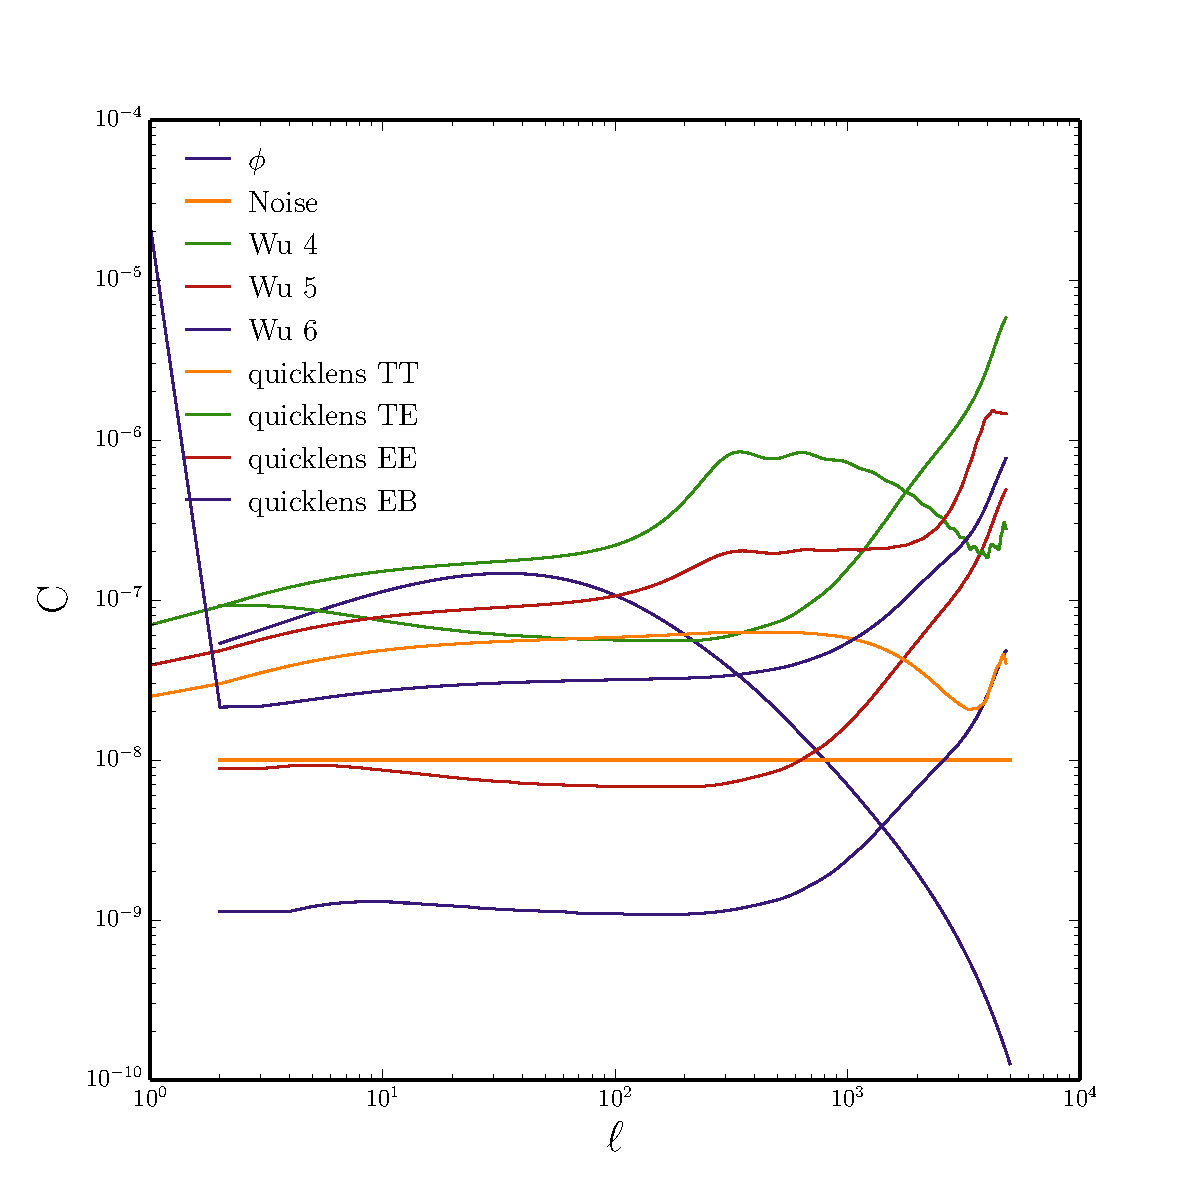
\includegraphics[scale=0.6]{PS_phi_with_noise.pdf}
\caption{Lensing potential power spectrum for our fiducial cosmology together with the lensing reconstruction noise $N^{\phi}$ used in this work.}
\label{fig:phi-cl-noise}
\end{center}
\end{figure}

\begin{figure}[htbp]
\begin{center}
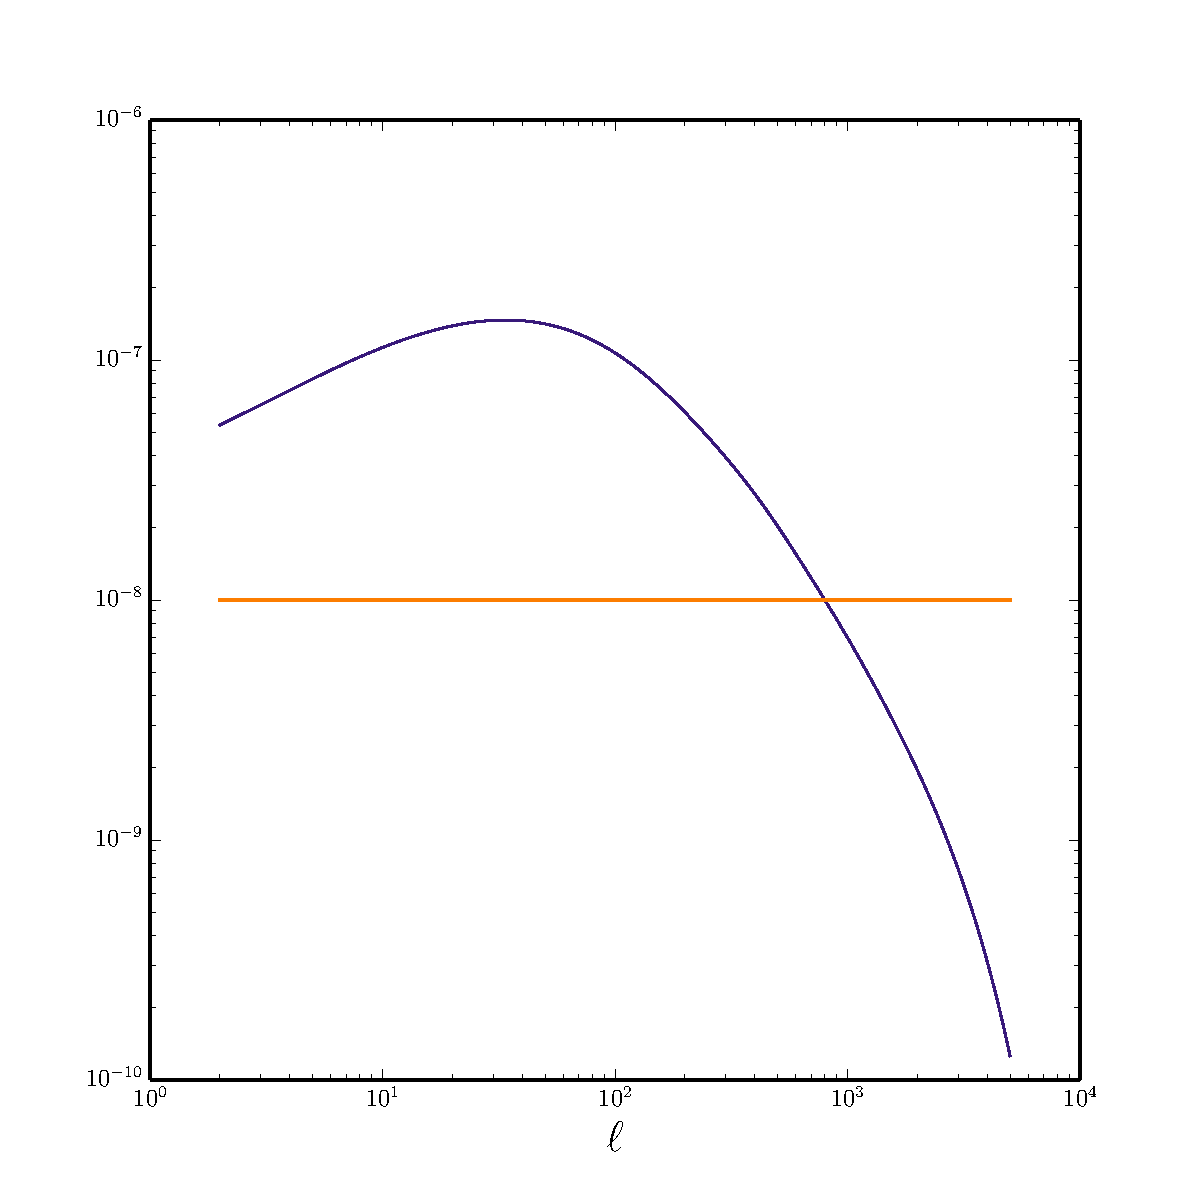
\includegraphics[scale=0.6]{PS_with_noise.pdf}
\caption{CMB power spectrum for our fiducial cosmology together with the instrumental noise used in this work. They are basically equivalent to a cosmic variance limited experiment with $l_{max}\sim 3000$}
\label{fig:cmb-cl-noise}
\end{center}
\end{figure}





\begin{eqnarray}
\centering
	s\ [\;\mu {\rm K.arcmin}\;] \equiv \frac{ {\rm NET}\ [\; \mu{\rm K.}\sqrt{s}\;] \times \sqrt{f_{sky} \ [\;{\rm arcmin}^2\;] }}{ \sqrt {N_{\rm det} \times Y \times \Delta T\ [\;{\rm s }\;]}}.
	\label{eq:sensitivity_definition}
\end{eqnarray}

\begin{equation}
	\centering
		F_{ij} \equiv - \left\langle\frac{\partial^2 \log \mathcal{L}}{\partial \theta_i \partial \theta_j} \bigg|_{\boldsymbol{\theta} = \boldsymbol{\theta_0}}\right\rangle
	\label{eq:Fij_def}
\end{equation}

 \begin{eqnarray}
 	\centering
		\mathbf{C}_\ell \equiv \left( \begin{array}{ccc}C_\ell^{TT} + N_\ell^{TT} & C_\ell^{TE} & C_\ell^{Td} \\ C_\ell^{TE} & C_\ell^{EE} + N_\ell^{EE} & 0 \\ C_\ell^{Td} & 0 & C_\ell^{dd} + N_\ell^{dd}\end{array}\right).
	\label{eq:cov_definition}
\end{eqnarray}

\begin{equation}
\sigma_i \equiv \sigma (\theta_i) = \sqrt{(\mathbf{ F^{-1}})_{ii}}
\end{equation}

\begin{equation}
F_{H_0 H_0} \rightarrow F_{H_0 H_0} + \frac{1}{(1\% \times H_{0,fid})^2}, 
\end{equation}


\begin{eqnarray}
	T_{\nu} = \left( \frac{4}{11} \right)^{1/3} T_{\gamma} 
	\label{eq:tnu_propto_tgamma}
\end{eqnarray}

\section{Data}

\begin{table}[htdp]
\caption{Fiducial values used.}
\begin{center}
\begin{tabular}{|c|c|}
\hline
$H_{0}$ &\\
\hline
\hline
$\tau$ &  \\
\hline

\hline
$A_{s}$ & \\
\hline

\hline
$n_{s}$ & \\
\hline

\hline
$N_{eff}$ & \\
\hline
\end{tabular}
\end{center}
\label{default}
\end{table}%


\section{Results}

\begin{table}[htdp]
\caption{How well we do constrain separate parameters with this data without any external prior?}
\begin{center}
\begin{tabular}{|c|c|}
\hline
$H_{0}$ & 0.32\% \\
\hline
\hline
$\tau$ & 2.26 \%\\
\hline

\hline
$A_{s}$ & 0.37 \%\\
\hline

\hline
$n_{s}$ & 0.25 \%\\
\hline

\hline
$N_{eff}$ & 0.9 \%\\
\hline

\end{tabular}
\end{center}
\label{default}
\end{table}%


\begin{figure}[htbp]
\begin{center}
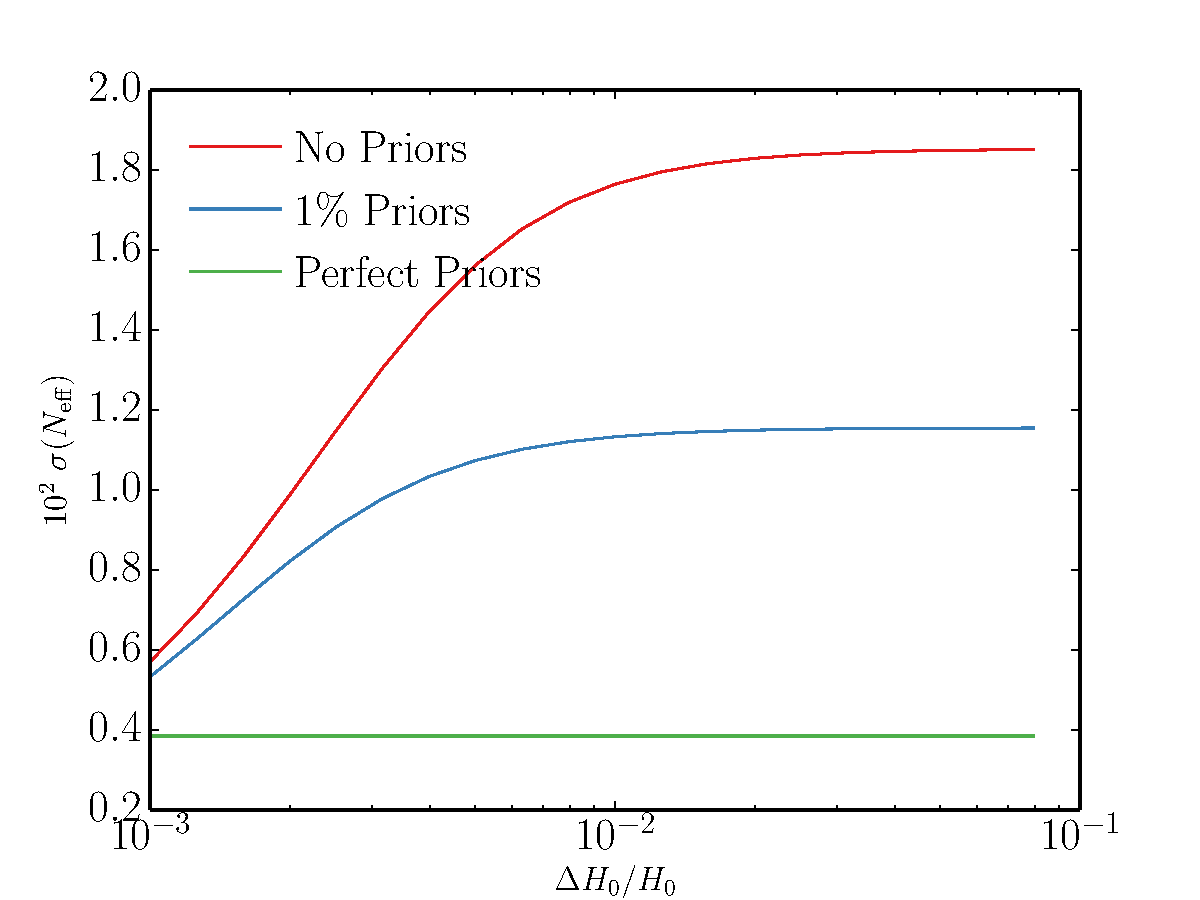
\includegraphics[scale=0.6]{h0_fisher.pdf}
\caption{}
\label{fig:phi-cl-noise}
\end{center}
\end{figure}

\begin{figure}[htbp]
\begin{center}
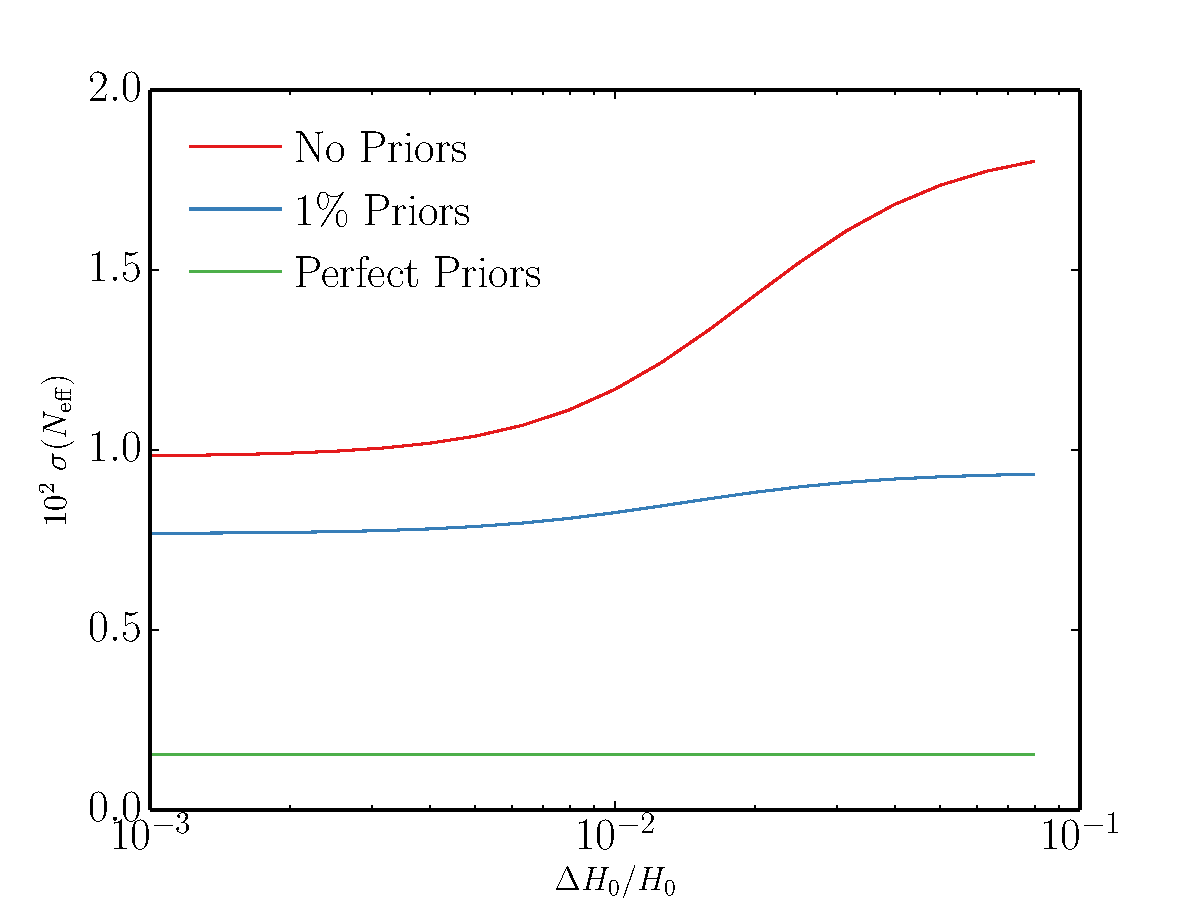
\includegraphics[scale=0.6]{tau_fisher.pdf}
\caption{}
\label{fig:phi-cl-noise}
\end{center}
\end{figure}



\section{Conclusions}



% If in two-column mode, this environment will change to single-column
% format so that long equations can be displayed. Use
% sparingly.
%\begin{widetext}
% put long equation here
%\end{widetext}

% figures should be put into the text as floats.
% Use the graphics or graphicx packages (distributed with LaTeX2e)
% and the \includegraphics macro defined in those packages.
% See the LaTeX Graphics Companion by Michel Goosens, Sebastian Rahtz,
% and Frank Mittelbach for instance.
%
% Here is an example of the general form of a figure:
% Fill in the caption in the braces of the \caption{} command. Put the label
% that you will use with \ref{} command in the braces of the \label{} command.
% Use the figure* environment if the figure should span across the
% entire page. There is no need to do explicit centering.

% \begin{figure}
% \includegraphics{}%
% \caption{\label{}}
% \end{figure}

% Surround figure environment with turnpage environment for landscape
% figure
% \begin{turnpage}
% \begin{figure}
% \includegraphics{}%
% \caption{\label{}}
% \end{figure}
% \end{turnpage}

% tables should appear as floats within the text
%
% Here is an example of the general form of a table:
% Fill in the caption in the braces of the \caption{} command. Put the label
% that you will use with \ref{} command in the braces of the \label{} command.
% Insert the column specifiers (l, r, c, d, etc.) in the empty braces of the
% \begin{tabular}{} command.
% The ruledtabular enviroment adds doubled rules to table and sets a
% reasonable default table settings.
% Use the table* environment to get a full-width table in two-column
% Add \usepackage{longtable} and the longtable (or longtable*}
% environment for nicely formatted long tables. Or use the the [H]
% placement option to break a long table (with less control than 
% in longtable).
% \begin{table}%[H] add [H] placement to break table across pages
% \caption{\label{}}
% \begin{ruledtabular}
% \begin{tabular}{}
% Lines of table here ending with \\
% \end{tabular}
% \end{ruledtabular}
% \end{table}

% Surround table environment with turnpage environment for landscape
% table
% \begin{turnpage}
% \begin{table}
% \caption{\label{}}
% \begin{ruledtabular}
% \begin{tabular}{}
% \end{tabular}
% \end{ruledtabular}
% \end{table}
% \end{turnpage}

% Specify following sections are appendices. Use \appendix* if there
% only one appendix.
%\appendix
%\section{}

% If you have acknowledgments, this puts in the proper section head.
%\begin{acknowledgments}
% put your acknowledgments here.
%\end{acknowledgments}

% Create the reference section using BibTeX:
\bibliography{basename of .bib file}

\end{document}




%
% ****** End of file apstemplate.tex ******

